\chapter{実装}
\label{chap:implementation}

本章では第\ref{chap:design}章で述べたシステムの設計を元にした、HypAR Touchの実装及び機能について述べる。

\newpage

\section{アプリケーション構成}
HypAR TouchはARナビゲーションを表示するモバイルアプリケーション、AR情報やNFC情報を永続化しAPIを提供するサーバー、Scrapbox、Gyazo\footnote{\textsf{https://gyazo.com}},NFCタグで構成される(図 \ref{fig:application_structure})。

\begin{figure}[h]
  \centering
  \includegraphics[width=150mm]{images/application_structure.jpg}
  \caption{構成図} \label{fig:application_structure}
\end{figure}

\subsection{HypAR Touchアプリ}
HypAR TouchアプリはReactNative\footnote{\textsf{https://reactnative.dev/}}と呼ばれるフレームワークを利用して作成されたモバイル端末アプリケーションである。
ReactNativeはWeb技術を利用し、マルチプラットフォームなネイティブアプリケーションを作成するためのフレームワークである。
このReactNative利用することでHypAR TouchアプリはAndroidとiOSの両方に対応したアプリケーションとなっている。

HypAr TouchアプリはNFCに記録された一意なidを取得し、そのidに紐付いた以下の情報を後述するHypAr Touchサーバーから取得する。
\begin{itemize}
  \item NFCタグの緯度経度
  \item NFCタグの設置される向き(0〜360度)
  \item 表示するAR情報の元となるScrapboxのプロジェクト名
  \item タッチした時に選択されているリンク情報
\end{itemize}
さらに取得したScrapboxのプロジェクト名をもとにHypAR TouchサーバーからARで表示する情報を取得する。
その上で取得したARの情報とNFCタグの緯度経度、NFCタグの設置された向きをもとに、各AR情報の位置を相対的に算出している。
また各AR情報には登録された位置付近で撮影されたパノラマ画像のURLが含まれている。
視点移動機能ではこのURLで登録された360度画像からVRのビューを作成している。

\subsection{HypAR Touchサーバ}
HypAR TouchサーバはNode.js\footnote{\textsf{https://nodejs.org/}}上で動作するWebアプリケーションとして実装されている。
HTTPリクエストを処理するWebアプリケーションフレームワークとしてExpress\footnote{\textsf{https://expressjs.com/}}を用い、
そのホスティング環境としてBaaS(Backend-as-a-Service)の1つであるHeroku\footnote{\textsf{https://www.heroku.com/}}を利用している。
HypAR TouchサーバはHypAR Touchアプリで利用するAR情報やNFCタグ情報を管理する役割をもっており、その機能は大きく4つに分けられる。

\begin{itemize}
  \item 対象となるScrapboxのプロジェクトをクロールし、AR表示に必要な情報を整理した上で永続化する。\\
  HypAR Touchサーバは指定されたScrapboxのプロジェクトを定期的にクロールし、位置情報やサムネイル画像のURL、リンク情報など、AR表示に必要な情報をまとめてデータベースに永続化している。
  これによりユーザがScrapboxに加えた変更がARでの表示に対応するようになっている。
  \\
  \item 登録されたNFCタグに関する情報を永続化する。\\
  NFCタグには一意なidが記録されており、それに紐づく形でタグの位置情報や向き、対象とするScrapboxプロジェクトなどの情報がこのサーバーに記録される。
  \\
  \item クロールした情報を元にパノラマ画像を生成し、Gyazoに保存した上でそのURLを記録する。\\
  第3章で記述した視点移動機能を実装するためにはARで表示する情報に加えて、記録された位置情報に最も近いところから撮影されたパノラマ画像が必要である。
  そのためHypAR TouchサーバではARで表示する情報ごとにGoogle Street ViewのAPI\footnote{\textsf{https://developers.google.com/maps/documentation/streetview/overview}}を利用してその地点からのパノラマ画像を生成している。
  また、画像の保存・永続化には後述するGyazoを利用しており、最終的にはGyazoに保存されたパノラマ画像のURLをARで表示する情報と合わせてデータベースに永続化している。
  \\
  \item 上記3つの情報を取得・追加・変更するAPIを提供する。\\
  HypAR Touchサーバは上記3つの情報を生成・永続化するだけでなく、HypAR TouchアプリからのAR情報取得やNFCタグの登録を受け付ける必要がある。
  そのためHypAR Touchサーバはこれらの情報を取得、追加、更新するAPIを提供している。

\end{itemize}

\subsection{Scrapbox}
Scrapbox(図\ref{fig:scrapbox})はGyazz\cite{Gyazz}をベースにして開発された、Nota\footnote{\textsf{https://www.notainc.com/ja}}社が運営しているWikiである。
本システムではこのScrapboxをARで表示する情報の管理ツールとして利用している。
これはScrapboxが他のシステムには存在しない以下のようなHypAR Touchに適した特徴を持つためである。
\begin{itemize}
  \item シンプルで柔軟な記法をもつWYSIWYGエディタ
  
  入力/改行/段落/箇条書きといった基本的なテキスト編集を見たまま行える。
  
  \item 場所指定に最適なLocation記法
  
  Google MapsのURLを貼り付けるだけで地図を埋め込めるLocation記法\footnote{\textsf{https://scrapbox.io/help-jp/Location記法}}と呼ばれる機能があり地理情報を記述するのに適している。
  本システムではこのLocation記法によって表示する情報の場所を指定している。

  \item リンク記法によるシンプルなハイパーリンクと関連ページリスト
  
  Scrapboxでは単語を\texttt{[]}で囲うだけで同一Wiki内ページへのリンクとすることが可能である。
  さらにScrapboxページの下部には
  \begin{itemize}
      \item 別ページへのリンク
      \item 別ページからのリンク
      \item リンク先ページがリンクしているページ
  \end{itemize}
  といった関連ページリスト(図\ref{fig:scrapbox_related})が表示され、どのような情報と関連するのかが一目瞭然に分かる。

\end{itemize}

\begin{figure}[h]
  \begin{minipage}{0.5\hsize}
    \centering
    \includegraphics[width=75mm]{images/scrapbox_screen.png}
    \caption{Scrapboxの画面} \label{fig:scrapbox}
  \end{minipage}
  \begin{minipage}{0.5\hsize}
    \centering
    \includegraphics[width=75mm]{images/scrapbox_related_screen.png}
    \caption{Scrapboxの関連ページリスト} \label{fig:scrapbox_related}
  \end{minipage}
\end{figure}
またScrapboxはプロジェクト内のページリストと各ページの情報を取得するAPI\footnote{\textsf{https://scrapbox.io/help-jp/API}}を持っており、これを利用することでHypAR TouchサーバはScrapboxをクロールしている。

\subsection{Gyazo}
Gyazoは、パソコンのデスクトップ画面の一部をキャプチャしてWebにアップロードするツールおよび画像を保存する画像/映像専用のクラウドストレージサービスである。
Gyazoには十分な保存容量があり、画像のアップロード・取得等のAPIも揃っている。
そのため自身のサーバよりも安全に画像を管理可能なGyazoを本システムでのパノラマ画像の保存先として利用している。

\subsection{NFCタグ}
本システムで利用するNFCタグはモバイル端末のOSに関わらず、読み込めるタグ形式とデータフォーマットでなくてはならない。
そのため本システムではNFCタグとして最も普及しているISO/IEC 14443 TypeAに準拠したNFCタグを利用している。
また同様にNFC FORUMが策定したデータフォーマットであるNDEFを利用することでNFC機能を持つほとんどのモバイル端末に対応している。
NDEFのデータ形式には更に細かく、Text、URI、SmartPostermの3つのタイプが存在する。
このうちURIタイプで書かれたNFCタグは殆どのNFC対応スマートフォンでのバックグラウンド読み取りに対応している。
またAndroidとiOSにはディープリンクと呼ばれる特殊なURIからインストールされたアプリケーションを起動する機能が存在しており、そのURIの形式をCustom URL Schemeと呼ぶ。
Custom URL Schemeでは図\ref{fig:custom_url_scheme}のように起動するアプリの指定だけでなく、URIパラメータを利用して追加の情報を記述しアプリケーション側にその情報を渡すことが可能である。
このような特徴を踏まえ、本システムではNFCタグにCustom URL Schemeの形にしたURIをNDEFのURIタイプとして記録している。
これにより、モバイル端末でNFCタグにタッチするだけでアプリの起動及びタグIDの受け渡しが可能となる。

\begin{figure}[h]
  \centering
  \includegraphics[width=150mm]{images/custom_url_scheme.jpg}
  \caption{Custom URL Scheme} \label{fig:custom_url_scheme}
\end{figure}

% \section{NFCによるキャリブレーション}
% NFCタグによって行われる位置推定の仕組みについて解説する。



\section{機能}

\subsubsection{HypAR Touchアプリによるナビゲーション閲覧}
\paragraph*{NFCタグにタッチする}
本アプリケーションは図\ref{fig:touch_nfc}のように専用の情報が書かれたNFCタグにタッチすることで起動し、ナビゲーションを開始する。
NFCにタッチすることで端末の位置と向きが認識され、図\ref{fig:hypar_touch_init_screen}のように登録された情報をARで正しい位置に表示することができる。
また画面下部にあるスライダー(図\ref{fig:hypar_touch_slider})を動かすことでARで表示する情報の距離の範囲を指定することができる。

\begin{figure}[h]
  \centering
  \includegraphics[width=100mm]{images/touch_nfc.jpg}
  \caption{NFCタグにタッチする様子} \label{fig:touch_nfc}
\end{figure}

\begin{figure}[h]
  \begin{minipage}{0.5\hsize}
    \centering
    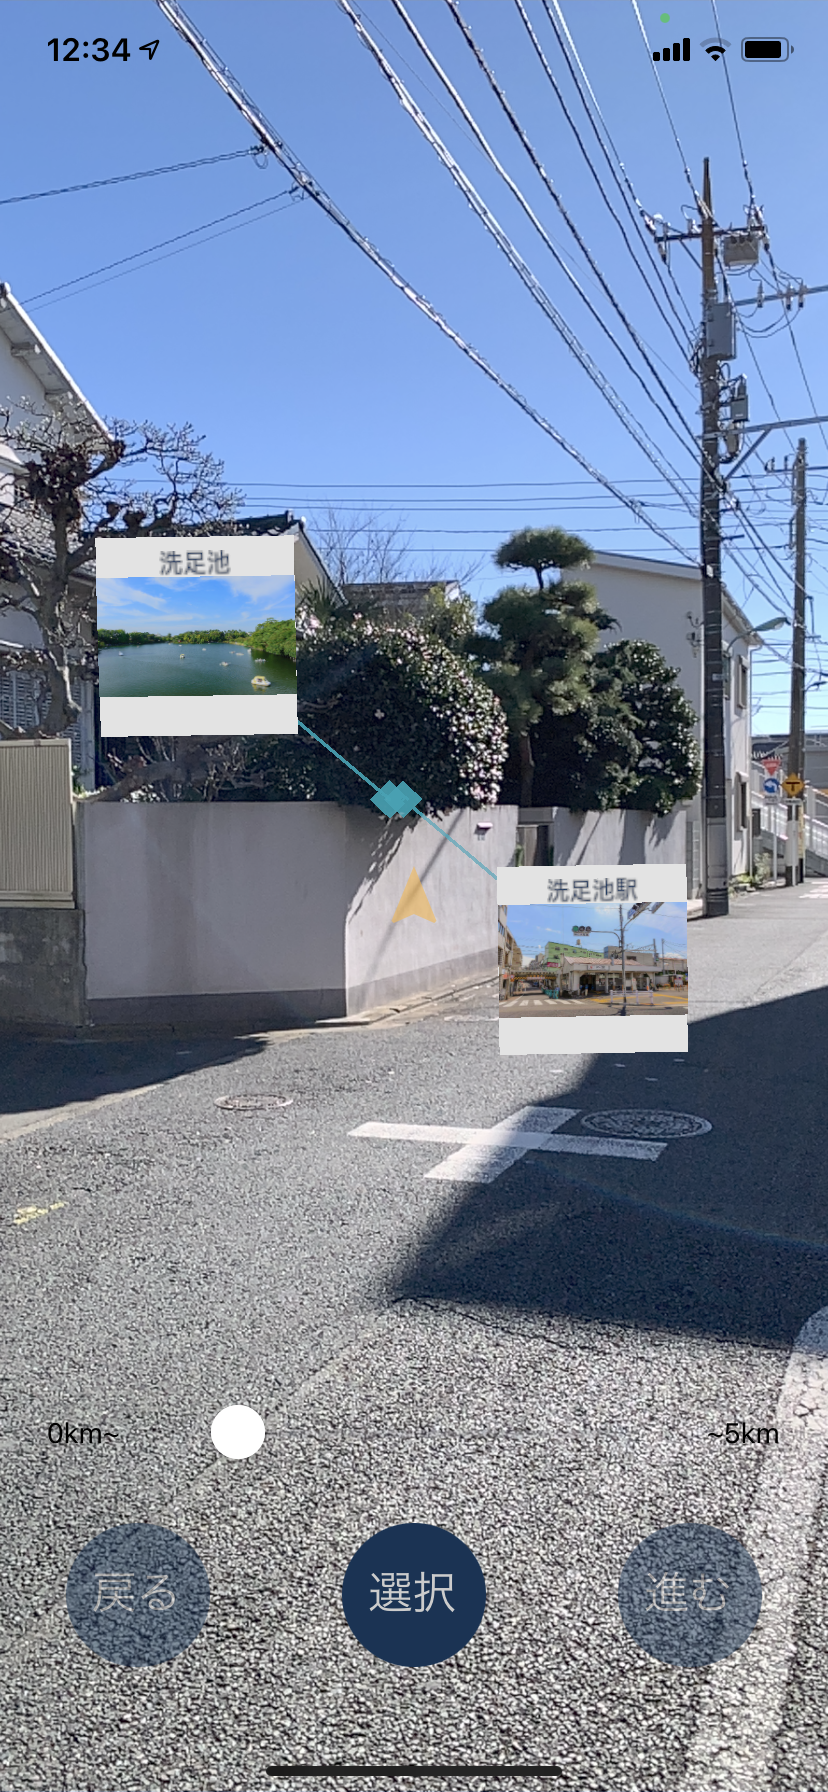
\includegraphics[height=100mm]{images/hypar_touch_init_screen.png}
    \caption{ARでの表示} \label{fig:hypar_touch_init_screen}
  \end{minipage}
  \begin{minipage}{0.5\hsize}
    \centering
    \includegraphics[height=100mm]{images/hypar_touch_slider.png}
    \caption{スライダーによる距離指定} \label{fig:hypar_touch_slider}
  \end{minipage}
\end{figure}

\paragraph*{表示されたAR情報の関連情報を表示・選択する}
画面の中央にはオレンジ色の三角のカーソルが表示されており、これをARで表示された情報の上に重ねると青い枠線が表示される(図\ref{fig:hypar_touch_hover})。
その状態で画面下部の選択ボタンを押すと図\ref{fig:hypar_touch_selected}のように関連する情報が放射状に配置されてに表示される。
これらの表示された関連情報も同じようにカーソルで選択することができる(図\ref{fig:hypar_touch_sub_selected})。
このように関連情報を選択していくことによって興味のある情報をAR上で探索することができる。

\begin{figure}[h]
  \begin{minipage}{0.5\hsize}
    \centering
    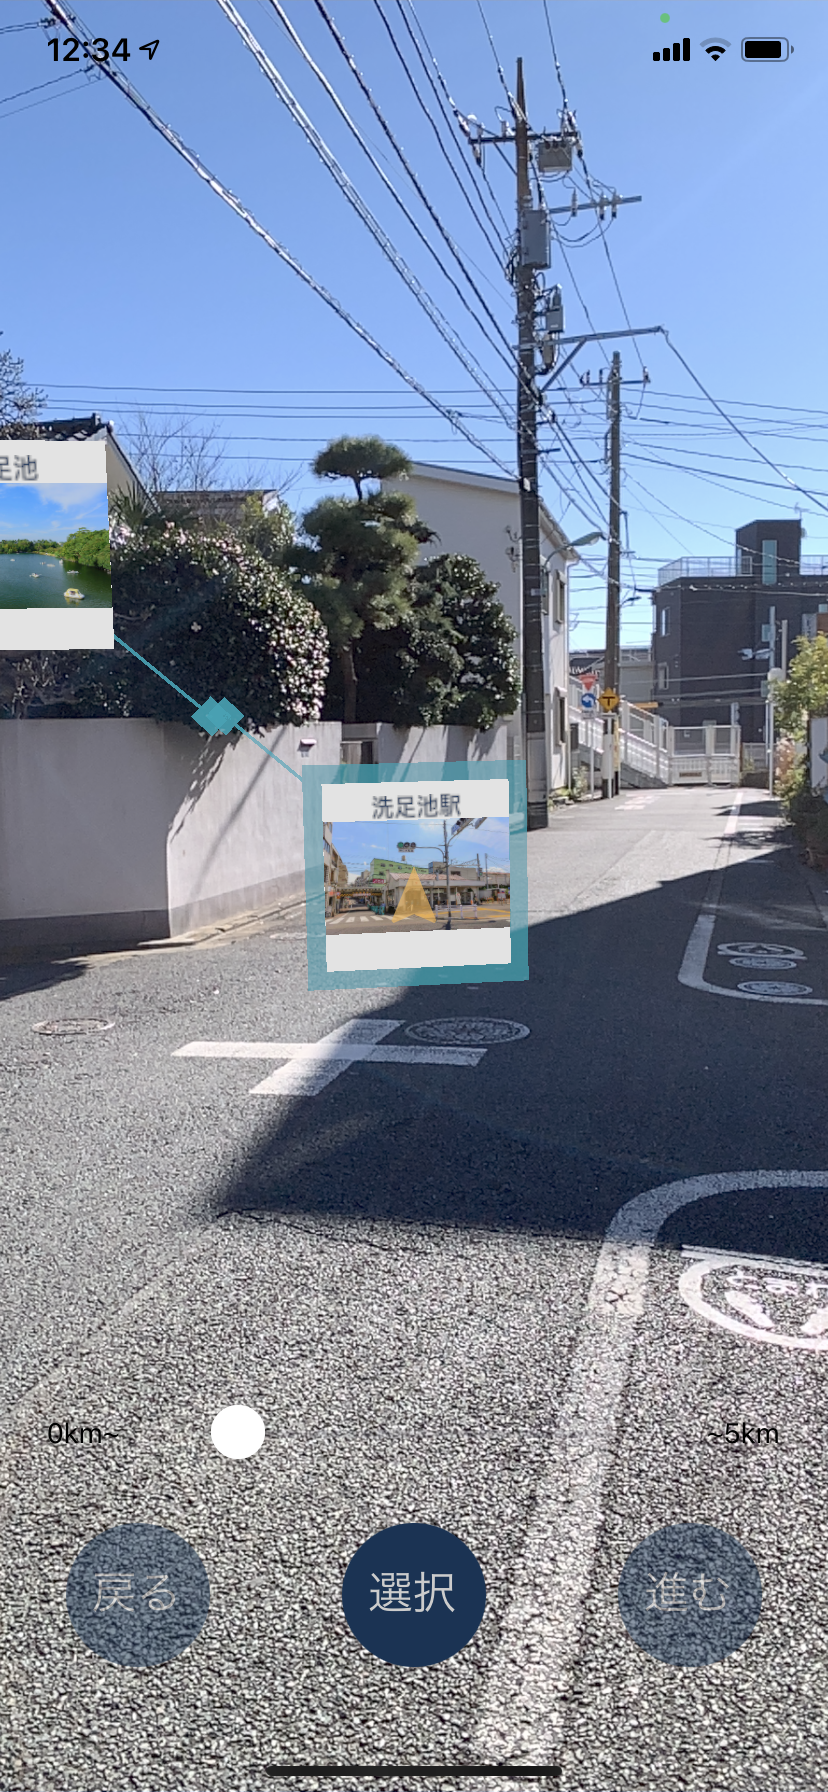
\includegraphics[height=100mm]{images/hypar_touch_hover.png}
    \caption{カーソルを重ねた状態} \label{fig:hypar_touch_hover}
  \end{minipage}
  \begin{minipage}{0.5\hsize}
    \centering
    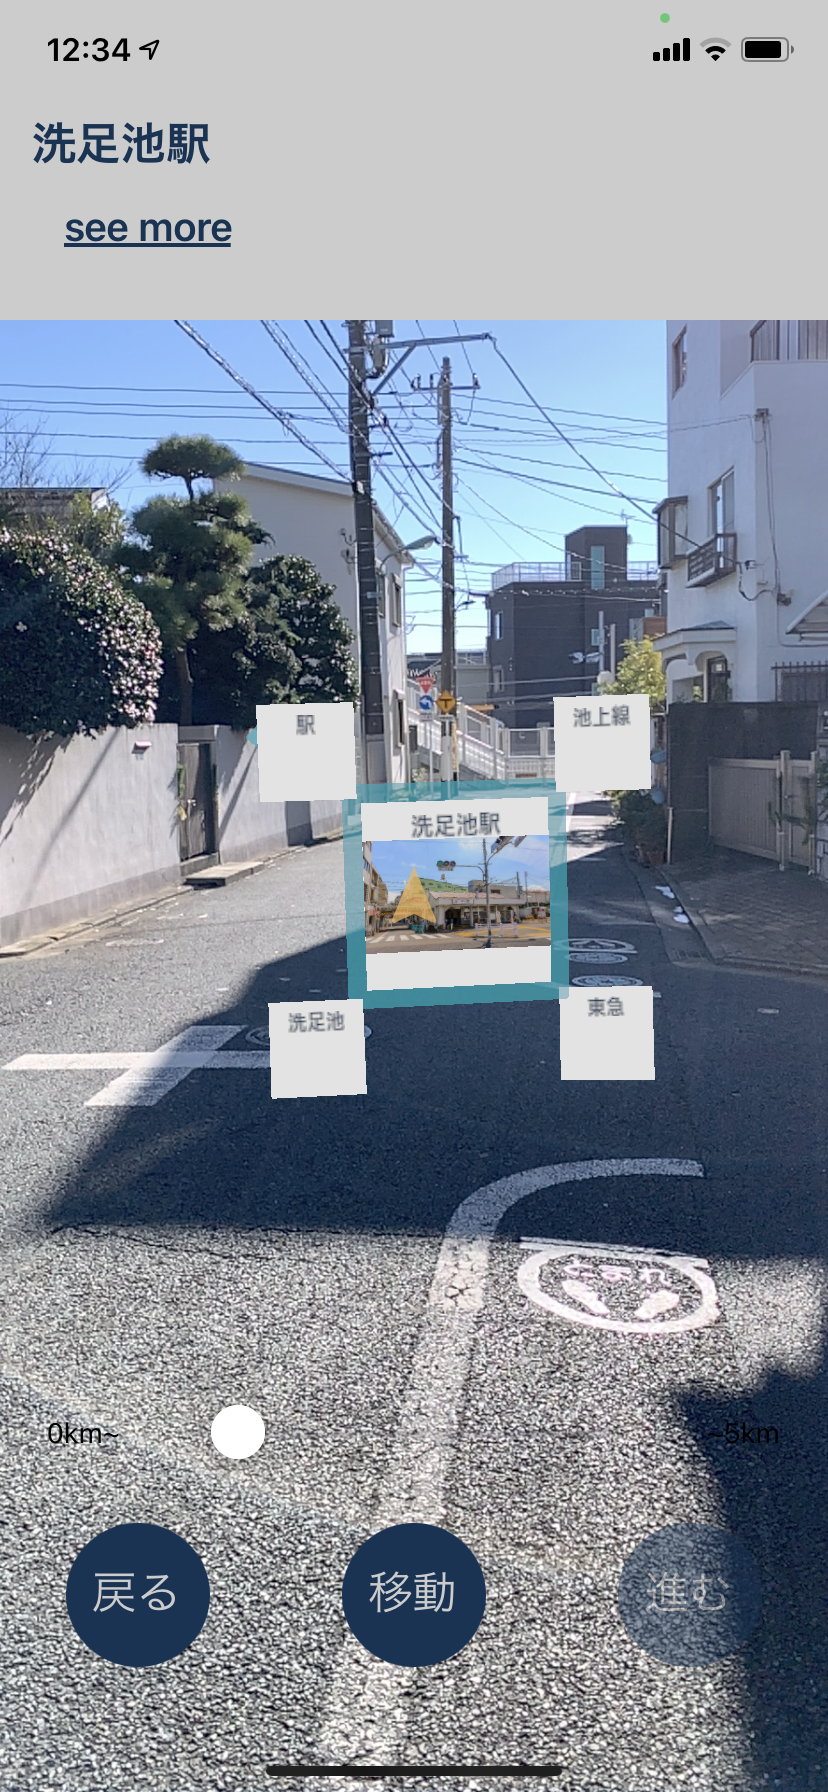
\includegraphics[height=100mm]{images/hypar_touch_selected.png}
    \caption{選択した状態} \label{fig:hypar_touch_selected}
  \end{minipage}
\end{figure}

\begin{figure}[h]
    \centering
    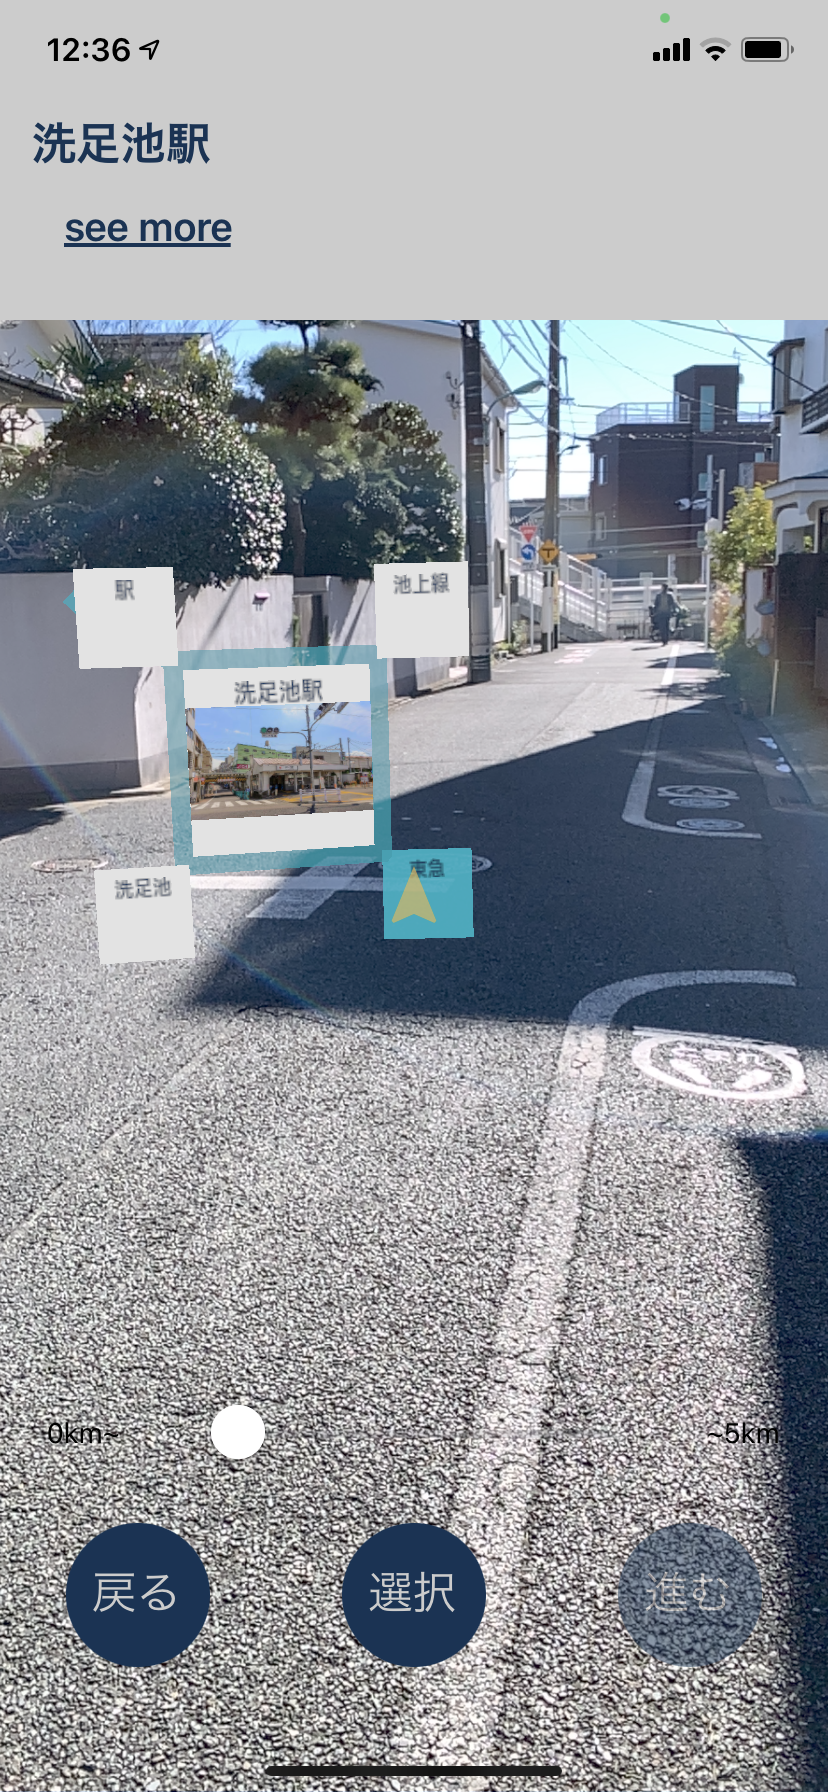
\includegraphics[height=100mm]{images/hypar_touch_sub_selected.png}
    \caption{関連情報の選択} \label{fig:hypar_touch_sub_selected}
\end{figure}


\paragraph*{選択されたAR情報の詳細を見る}
上記のようにカーソルをAR情報にあわせた上で選択ボタンを押すと画面上部には図\ref{fig:hypar_touch_top}のように選択された情報のタイトルの他に「see more」と書かれたボタンが出現する。
これをクリックすることでAR情報の元となったScrapboxをみることが可能である(図\ref{fig:hypar_touch_webview})。

\begin{figure}[h]
  \begin{minipage}{0.5\hsize}
    \centering
    \includegraphics[height=100mm]{images/hypar_touch_top.png}
    \caption{詳細を表示するボタン} \label{fig:hypar_touch_top}
  \end{minipage}
  \begin{minipage}{0.5\hsize}
    \centering
    \includegraphics[height=100mm]{images/hypar_touch_webview.png}
    \caption{Scrapboxでの情報表示} \label{fig:hypar_touch_webview}
  \end{minipage}
\end{figure}

\paragraph*{選択されたAR情報の場所に視点を移動する}
同じようにカーソルをAR情報にあわせた上で選択ボタンを押し、もう一度選択したAR情報にカーソルを重ねると画面下部中央のボタンが「移動」に変化する(図\ref{fig:hypar_touch_move_button})
この移動ボタンを押すと図\ref{fig:hypar_touch_move_map}のような地図での移動アニメーションを経て、選択した情報のある場所からの視点(図\ref{fig:hypar_touch_moved})に切り替えることができる。

\begin{figure}[h]
  \begin{minipage}{0.5\hsize}
    \centering
    \includegraphics[height=100mm]{images/hypar_touch_move_button.png}
    \caption{移動ボタン} \label{fig:hypar_touch_move_button}
  \end{minipage}
  \begin{minipage}{0.5\hsize}
    \centering
    \includegraphics[height=100mm]{images/hypar_touch_move_map.png}
    \caption{Mapでの移動アニメーションの途中} \label{fig:hypar_touch_move_map}
  \end{minipage}
\end{figure}

\begin{figure}[h]
  \centering
  \includegraphics[height=100mm]{images/hypar_touch_moved.png}
  \caption{移動先からの視点} \label{fig:hypar_touch_moved}
\end{figure}

\paragraph*{AR情報の選択を解除する・前の状態に戻る}
上記のような選択状態は画面の何も表示されていない部分をタップすることで解除できる。
また選択や移動した履歴情報は常に保存されており、画面下部の「戻る」「進む」ボタン(図\ref{fig:hypar_touch_history_button})で履歴を参照することができる。

\begin{figure}[h]
  \centering
  \includegraphics[height=100mm]{images/hypar_touch_history_button.png}
  \caption{進むボタンと戻るボタン} \label{fig:hypar_touch_history_button}
\end{figure}

\subsubsection{ScrapboxによるAR情報法の追加・編集}
HypAR Touchアプリに表示されるAR情報はNFCタグで指定されたScrapboxのプロジェクトをもとに生成される。
Scrapboxのプロジェクトにあるページのうち、Location記法によって位置情報の記述のあるページがアプリ側で表示されるAR情報と対応する。

\paragraph*{ARで表示する情報を追加する}
AR情報はScrapboxのページと対応しているため、新しくページを作成し、以下の2点の情報を記入することでAR情報が登録される。
\begin{itemize}
  \item ページタイトル
  
  図\ref{fig:scrapbox_ar_new}の\textcircled{\scriptsize{1}}部分であり、ページを作る上で必須となる項目である。
  このタイトルはHypAR Touchアプリ側でサムネイルとともにAR表示される。

  \item Location記法による記述
  
  Scrapboxにはソースコード \ref{google_map_url}のようなGoogle MapsのURLをソースコード \ref{location}のようなLocation記法に変換し、図\ref{fig:scrapbox_ar_new}の\textcircled{\scriptsize{2}}のようにマップとして表示する機能がある。
  この機能を利用し、AR情報を追加したい場所を中心としたGoogleMapのURLをScrapboxに貼り付けることでAR上で表示する場所を指定する。

  \begin{lstlisting}[caption=googleMapのURL, label=google_map_url]
    https://www.google.com/maps/place/%E6%9D%B1%E4%BA%AC%E9%A7%85/@35.681502,139.7671784,17z/data=!4m5!3m4!1s0x60188bfbd89f700b:0x277c49ba34ed38!8m2!3d35.6812362!4d139.7671248
  \end{lstlisting}

  \begin{lstlisting}[caption=Location記法, label=location]
    [N35.681502,E139.7671784,Z16 東京駅]
  \end{lstlisting}
\end{itemize}

\begin{figure}[h]
  \centering
  \includegraphics[width=120mm]{images/scrapbox_ar_new.png}
  \caption{新しくページを作成した時} \label{fig:scrapbox_ar_new}
\end{figure}

\paragraph*{サムネイルを追加する}
Scrapboxでは画像のURLを\texttt{[]}で囲う、または画像をドラッグ・アンド・ドロップすることで図\ref{fig:scrapbox_thumbnail}のようにページに画像を表示させることができる。
このようにScrapboxのページに画像を貼ると、ページの一番上にある画像がAR表示でのサムネイルになる。(図\ref{fig:scrapbox_thumbnail_and_ar})

\begin{figure}[h]
  \centering
  \includegraphics[width=120mm]{images/scrapbox_thumbnail.png}
  \caption{Scrapboxに貼り付けた画像} \label{fig:scrapbox_thumbnail}
\end{figure}

\begin{figure}[h]
  \centering
  \includegraphics[width=120mm]{images/scrapbox_thumbnail_and_ar.png}
  \caption{Scrapbox上の画像とARでの表示} \label{fig:scrapbox_thumbnail_and_ar}
\end{figure}

\paragraph*{ハイパーリンクを利用して説明を書く}
Scrapboxでは単語を\texttt{[]}で囲うことにより同一Wiki内ページへのハイパーリンクとすることが可能である。
他ページヘのハイパーリンクが生成されるとAR上で関連情報として表示されるようになる(図\ref{fig:scrapbox_link_and_ar})。
ARで表示したい情報の説明を書き、説明文中の単語を積極的にハイパーリンクにすることで関連する情報を提示することができる。

\begin{figure}[h]
  \centering
  \includegraphics[width=120mm]{images/scrapbox_link_and_ar.jpg}
  \caption{Scrapbox上のリンクとARでの表示} \label{fig:scrapbox_link_and_ar}
\end{figure}

\subsubsection{NFCタグに対する情報の書き込み}
NFCタグにはISO/IEC 14443 TypeAに準拠したNTAGを利用する。
また情報を記録する際にはNFC FORUM\footnote{\textsf{https://nfc-forum.org}}によって標準化されているNDEFフォーマットで情報を書き込む。
書き込む情報は図\ref{fig:nfc_uri}のようにCustomURLSchemeに沿ったURIの形式で書き込む。

\begin{figure}[h]
  \centering
  \includegraphics[width=120mm]{images/nfc_uri.png}
  \caption{NFCに書き込むURIデータ} \label{fig:nfc_uri}
\end{figure}

その上でタグに書き込んだIDと紐付ける形でHypAR Touchのサーバーに以下の情報を登録する。
\begin{itemize}
  \item 緯度経度
  \item タグの設置される向き(0〜360度)
  \item 表示するAR情報の元となるScrapboxのプロジェクト
  \item タッチした時に選択されているリンク情報
\end{itemize}
これらの情報はHypAR Touchアプリ内の登録画面(図\ref{fig:nfc_register_mobile})により登録可能である。

\begin{figure}[h]
  \centering
  \includegraphics[width=70mm]{images/nfc_register_mobile.png}
  \caption{モバイルアプリでの登録} \label{fig:nfc_register_mobile}
\end{figure}
